\documentclass[fontsize=12pt]{article}
\linespread{1.5}
% \usepackage[margin=2.5cm]{geometry}
\usepackage[margin=2.5cm, headheight=0pt, headsep=1cm]{geometry}
\usepackage{enumerate, fancyhdr, graphicx, amsmath, float, subcaption, textcomp, hyperref}

\usepackage[binary-units=true]{siunitx}
\sisetup{load-configurations = abbreviations}

\title{Old School \tetris{} Meets Page Rank}
\author{Paul Chesnais (pmc85) \& Sam ``Sven'' Svenningsen (sjs382)}
\date{}

\def\tetris{Tetris\textsuperscript{\textregistered}}

\pagestyle{fancy}
\fancyhead{}
\lhead{pmc85 \& sjs382}
\chead{Old School \tetris{} Meets Machine Learning}
\rhead{\tetris{}}
\fancyfoot{}
\rfoot{\thepage}
\lfoot{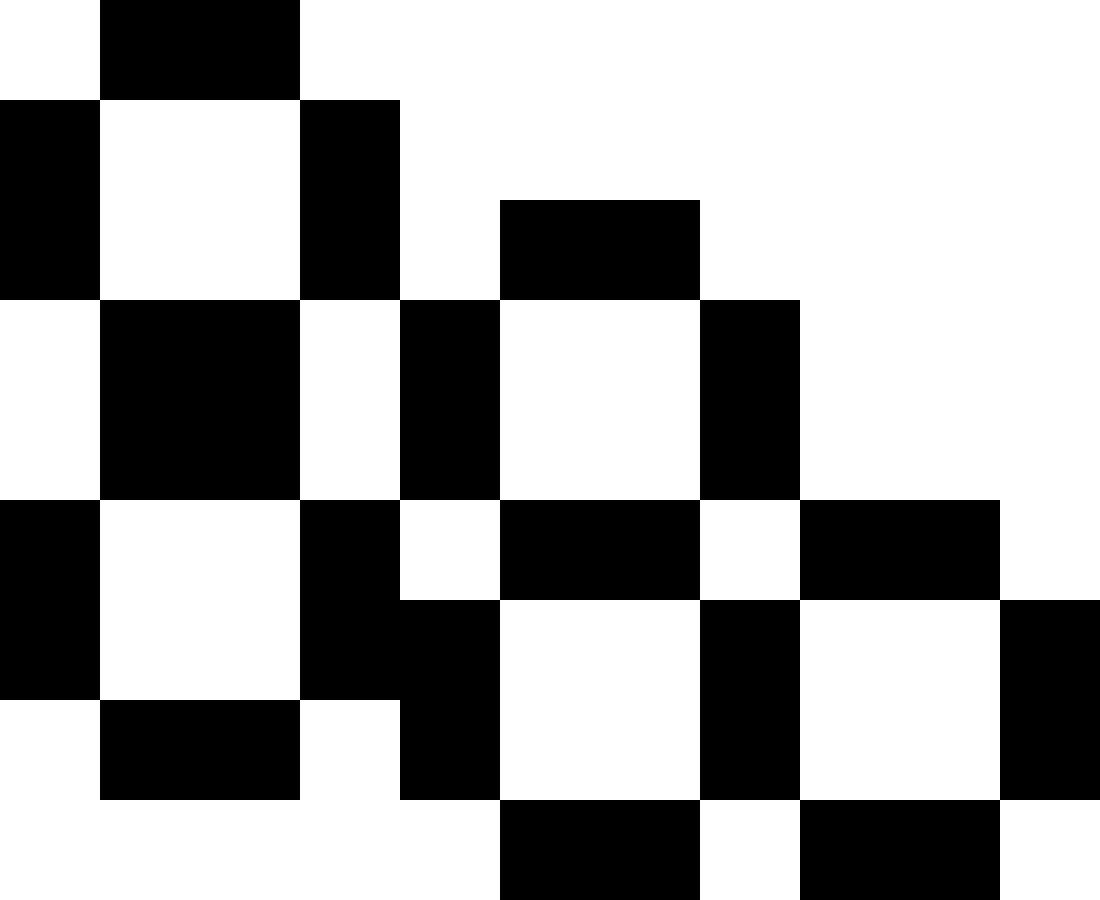
\includegraphics[height=20pt]{Logo}}
\renewcommand{\headrulewidth}{0.5pt}
\renewcommand{\footrulewidth}{0.5pt}

\usepackage{listings, color, times, textcomp, setspace}
\definecolor{Code}{rgb}{0,0,0}\definecolor{Decorators}{rgb}{0.5,0.5,0.5}\definecolor{Numbers}{rgb}{0.5,0,0}
\definecolor{MatchingBrackets}{rgb}{0.25,0.5,0.5}\definecolor{Keywords}{rgb}{0,0,1}\definecolor{self}{rgb}{0,0,0}
\definecolor{Strings}{rgb}{0,0.63,0}\definecolor{Comments}{rgb}{0,0.63,1}\definecolor{Backquotes}{rgb}{0,0,0}
\definecolor{Classname}{rgb}{0,0,0}\definecolor{FunctionName}{rgb}{0,0,0}\definecolor{Operators}{rgb}{0,0,0}
\definecolor{Background}{rgb}{0.98,0.98,0.98}

\lstdefinestyle{Scala}{
  backgroundcolor=\color{Background},basicstyle=\ttfamily\small\setstretch{1},breaklines=true,commentstyle=\color{Comments}\slshape,emph={self},emphstyle={\color{self}\slshape},frame=l,framexbottommargin=2em,framextopmargin=2em,keywordstyle={[2]\color{Decorators}\slshape},keywordstyle={\color{Keywords}\bfseries},morekeywords={abstract,case,catch,class,def,do,else,extends,false,final,finally,for,if,implicit,import,lazy,match,mixin,new,null,object,override,package,private,protected,requires,return,sealed,er,this,throw,trait,true,try,type,val,var,while,with,yield},otherkeywords={=>,<-,<\%,<:,>:,\#,@},sensitive=true,morecomment=[l]{//},morecomment=[n]{/*}{*/},morestring=[b]",morestring=[b]',morestring=[b]""",numbers=left,numbersep=1em,numberstyle=\footnotesize,showspaces=false,showstringspaces=false,showtabs=false,stringstyle=\color{Strings},tabsize=4,xleftmargin=1em,
}

\begin{document}
\maketitle
\thispagestyle{empty}
\section{Abstract}
\label{sec:abstract}

\par It has been shown that \tetris{}, the Russian tile-stacking puzzle video game, is NP-Complete \cite{bib:tetrishard}. This project sought to try to approximate a solution to \tetris{} that plays well according to human standards. Evidently, no solutions can be perfect (assuming $P \neq NP$), but one can still try. The current algorithm approximates a solution by ranking the contour (the shape of the top of the stack) using a method akin to Google's PageRank algorithm, then choosing the sequence of Tetrominoes (\tetris{} pieces) that lead to the highest ranking stack.

\section{Getting computers to play \tetris{}}
\label{sec:getting_computers_to_play_tetris}

\subsection{An Introduction to the Game}
\label{sub:an_introduction_to_the_game}

\begin{figure}[h!]
  \centering
  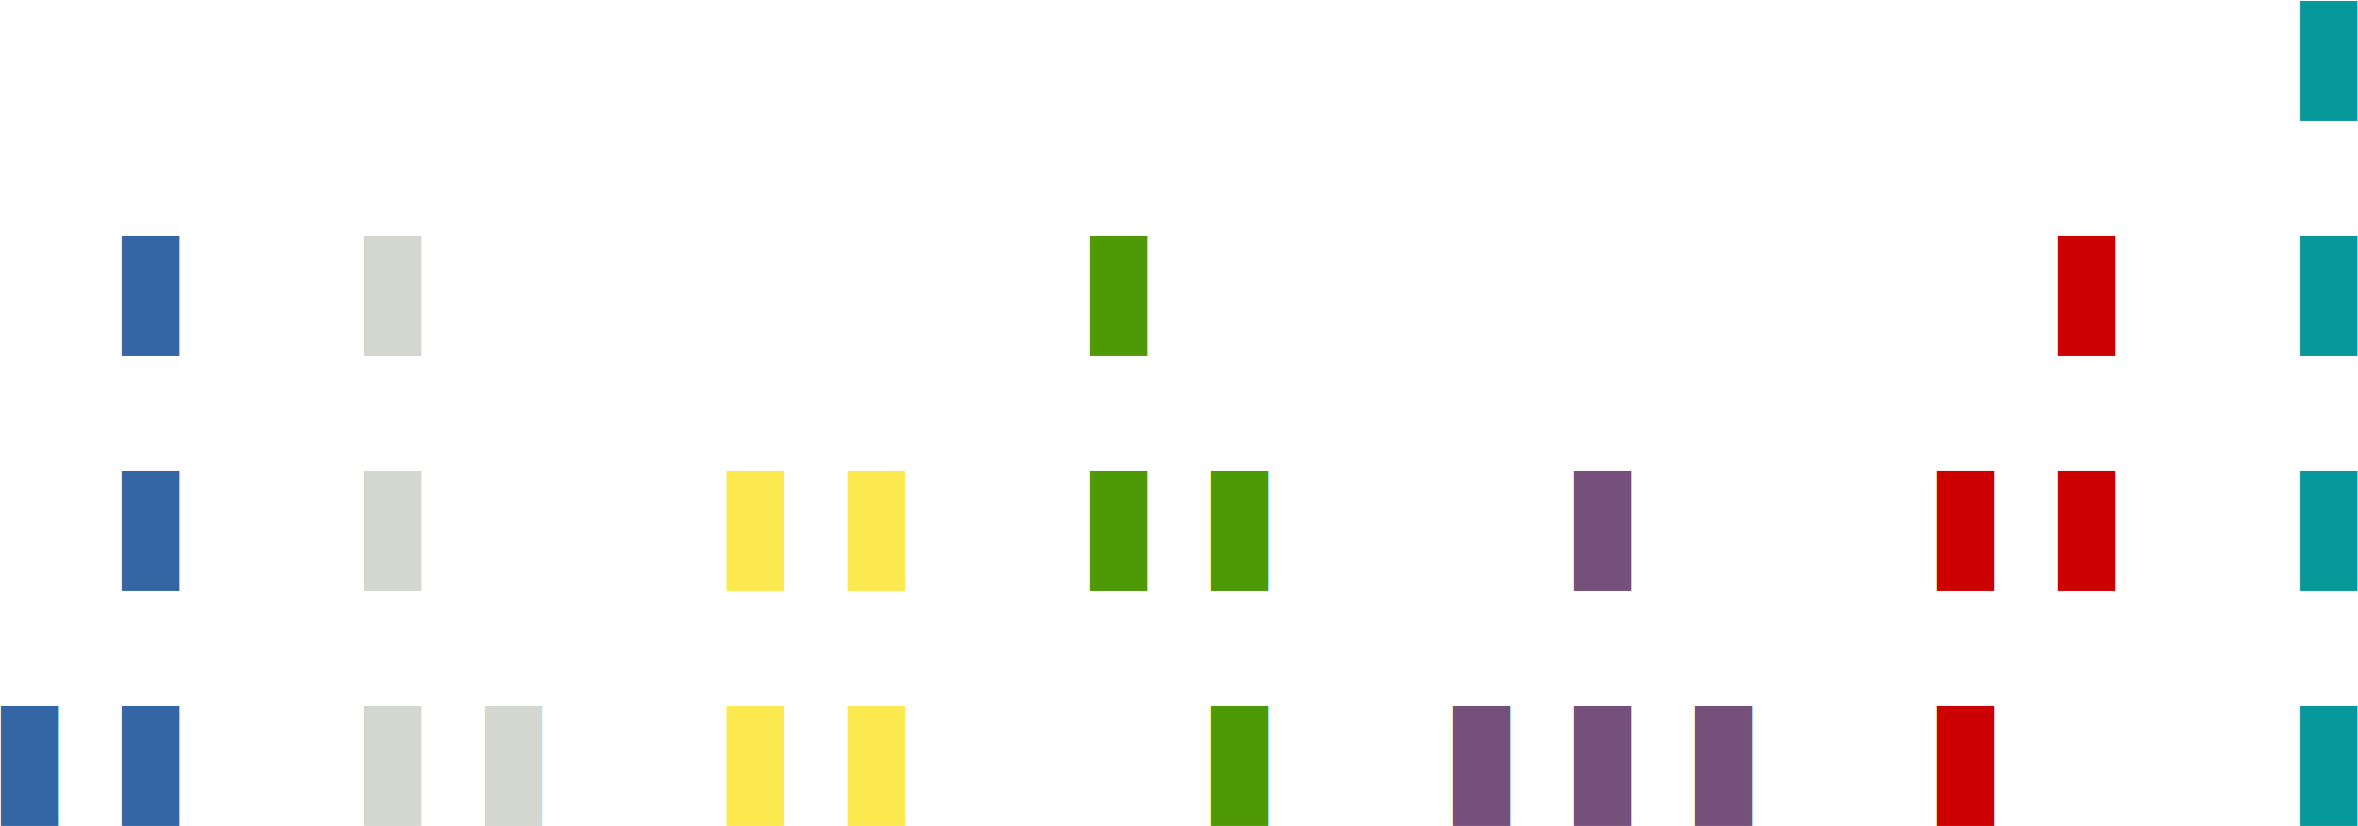
\includegraphics[width=0.4\textwidth, height=0.1\textwidth]{figures/pieces}
  \caption{The 7 tetrominoes J, L, O, S, T, Z and I }
  \label{fig:the_7_tetrominoes}
\end{figure}

\par The mechanics of \tetris{} are beautifully simple. The user begins with an game board, henceforth referred to as the ``stack'', 10 units wide and 20 units high. The user is then given a random sequence of the \tetris{} pieces, or ``tetrominoes'', shown in Figure~\ref{fig:the_7_tetrominoes}, to be placed on top of one another. Tetrominoes are each made up of 4 identical connected squares, and rotate by 90\textdegree clockwise or counterclockwise. When a tetromino is placed, it maintains its shape. In other words, it can create holes (see Figure~\ref{fig:placing_an_i_piece_to_clear_a_row}).
\par When a horizontal line is full, this line is removed. Every individual square above the cleared row then move directly downward $n$ vertical units, where $n$ is the number of row cleared. Figure~\ref{fig:placing_an_i_piece_to_clear_a_row} shows both the mechanic involved in clearing rows, and how poor placement of piece can create undesired holes. Here, the I piece was placed horizontally on top of the O, which blocks access to the three empty spaces below.
\par As time goes on, the amount of time the user has to place the piece decreases, making it difficult to keep up with, and to keep playing, the user must clear as many rows as possible to prevent the top of the stack from reaching height 20, otherwise, it's GAME OVER. The game is scored relative to how many rows were cleared by a single placement, and how frequently rows are cleared. The best score is achieved by using the I piece to clear 4 rows at once, and consecutive row clears multiply the score given (i.e. combos).

\begin{figure}[h!]
  \centering
  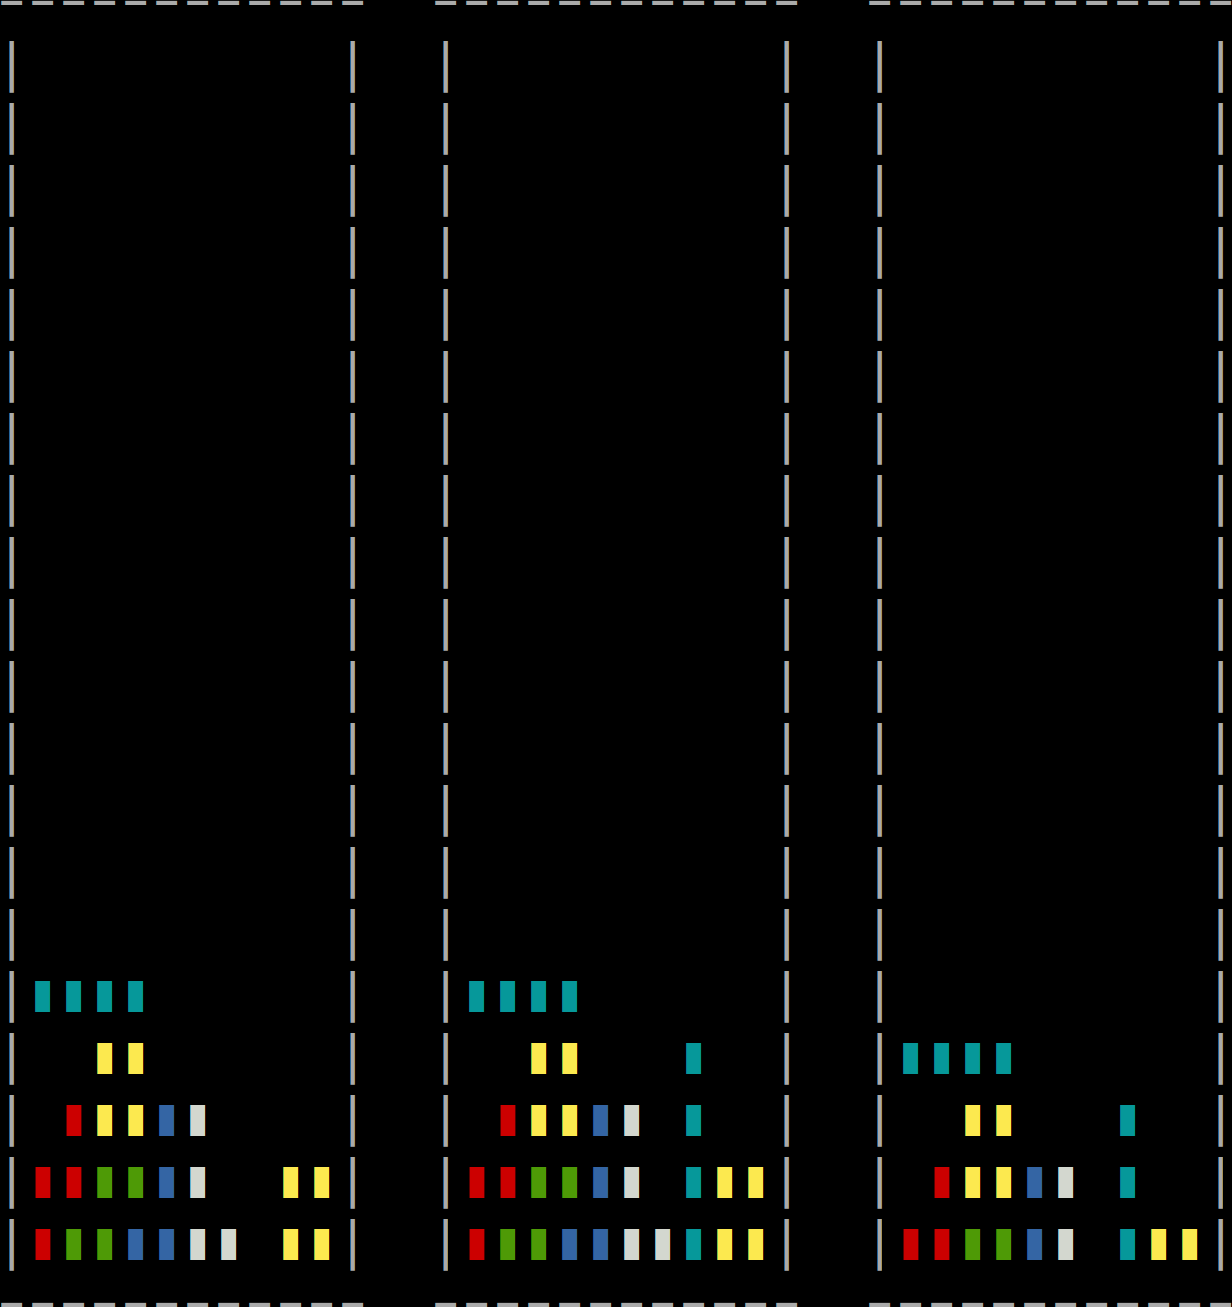
\includegraphics[width=0.6\textwidth, height=0.4\textwidth]{figures/rowclear-crop}
  \caption{Placing an I piece to clear a row}
  \label{fig:placing_an_i_piece_to_clear_a_row}
\end{figure}

\subsection{Representations}
\label{sub:representations}
\subsubsection{Tetrominoes}
\label{ssub:tetrominoes}

\par A simple, yet efficient efficient way to represent an single rotation of an individual tetromino is by keeping a list of two dimensional vectors representing the location of each square from the center of mass of the tetromino. Equation~\ref{eq:t_offsets} is an example of such a list for the T piece in the orientation shown in Figure~\ref{fig:the_7_tetrominoes}.
\begin{align}
  [(0,0), (-1, 0), (0, 1), (1, 0)]\label{eq:t_offsets}
\end{align}
With these lists and a given pair of coordinates $(x,y)$, finding the location of each square of a given tetromino only requires translating $(x,y)$ by each vector in the list.

\subsubsection{The Stack}
\label{ssub:the_stack}
\subsubsection{Arrays}
\label{ssub:arrays}
\par One way to represent a stack is with an array. In this case, the stack was represented as a $10\times 20$ two dimensional array, where each square in the theoretical stack maps to an element in the array. One square is represented as a tuple $(s,c)$ where $s$ is a boolean representing whether or not there exists a square in the stack at that location, and $c$ is the color of that square \footnote{Again, $c$ is only kept for graphical purposes and plays no role in the actual implementation}. In this implementation, traversing the array to figure out whether or not a row is full is very straightforward.
\par Adding a tetromino to such a stack is a little more difficult. The player (human or otherwise) only has a choice between which column the center of mass of the tetromino will fall on, and at which height the piece will settle is entirely dependent on the current state of the stack. To find which height the tetromino should settle at, all we need to do is iteratively try to place the tetromino higher and higher starting at the current height of the specified column plus one. If at any time, any of the squares in the tetromino occupy a square that is already full, this height must be invalid, and we must try again one unit higher. Once all the squares fit and occupy what were empty spaces, return the new stack. This is a little slow, but is the only way to find a position where the tetromino fits.
\subsubsection{Contour}
\label{ssub:contour}
\par The other way to represent a stack, according to Ryan Heise's similar attempt at playing \tetris{} \cite{bib:ryan_heise}, is by only keeping track of the shape of the stack's contour. The stack's contour is defined by the height of each individual column minus the height of the shortest column. Suppose we maintain the guarantee that the stack is always full, i.e. never has holes, and one of the outermost columns is always kept empty. In this case, two stacks of different heights can have the same contour, and all stacks with the same contour can be treated equally. Heise also introduced a method of serializing this contour to a single integer. A stack can be represented as a sequence of ``relative difference in height between one column and the next'', with the slight subtlety that an absolute difference greater than 4 will be cut to -4 and 4 accordingly. This sacrifice in complexity is argued to be mostly harmless under the guise that two such stacks will behave similarly. Given this sequence of numbers between -4 and 4, we can add 4 to each and string them together to get a base 9 integers. There is therefore a 1 to 1 mapping between contours and integers, which allows us to hash the contour.
\par We can also add tetrominoes directly to a contour, given a desired column. First, transform the contour back into a list of heights. Then, for the desired column, attempt to place the tetromino at that height plus the height of the tetromino's center of mass. For all columns of height $h$, if the tetromino adds $n$ squares to that column, check that all those squares are at height $\leq h + n$. If not, then placing the tetromino at that height must have put a hole in the stack. This violates the invariant that a contour represents a stack with no holes, and therefore that tetromino cannot be placed in this spot. This is more efficient than the addition operation described above, since there are fewer squares to check.

\subsection{Relaxations}
\label{sub:relaxations}
\begin{description}
  \item[Scoring] The scoring scheme outlined above is unfortunately quite complex. Additionally, every implementation of \tetris{} uses a slightly different scheme. As such, given that there is no strong consensus and given the additional complexity, the decision was made to score a player by how many tetrominoes they can consecutively place without losing. This also implies that a bot can search for the best move only by looking at the expected life of the stack that it creates.
  \item[Timing] Another important aspect of \tetris{} is that there is a time limit for every move. The first problem is that it is hard to interrupt a running algorithm and get the currently computed best move from it. The second problem is that computers are quite fast, and are expected to come up with the next best move rather quickly. As such, instead of setting arbitrarily low time limits on the players, no time limits were set under the assumptions that AI players would be too fast for it to matter anyway.
\end{description}

% \subsection{The Motivation}
% \label{sub:the_motivation}
% Some scientists have shown that \tetris{} is NP-Complete. In other words, there exists


\section{Initial Attempts}
\label{sec:initial_attempts}

\subsection{MiniMax}
\par We tried to maximize the pieces placement in a way that would minimize the possible damage/maximize the least expected outcome of the next few pieces the \tetris{} board provides by using the MiniMax approach.
\subsubsection{Heuristic}
\par This lead us into the difficulty of grading boards on quality so that we could have a function to minimize over.

\par One thought would be to penalize boards that have holes or overhangs in them (i.e. pieces covering empty spaces), though penalize overhangs less since you can get around them sometimes.

\par The next obvious criteria was to give a max value to any board that has a \tetris{} (4 complete rows at once) and a lesser, but still high, score to any number of complete rows.

\par This leaves us an issue of all the boards with no obvious issues, and no obvious bonuses. We made a guess that having a more level board would be best (i.e. the distance between the lowest free spot and the highest tower you have is minimized).

\par An alternative to this is to make up as many features as possible and try to assign weights to them based on if they lead to failed games quickly (we'd have to play the game a bunch of times).

\par We weren't quite sure how to implement this though since we did not know how to weight each feature appropriately besides running it a million times over, which was too slow.

\subsubsection{The Tree}

\par We began by choosing trees that would be good regardless of what the unknown pieces would be, this meant leaving out what would probably have been good choices assuming we didn't get the one or two pieces, or combinations, that messed it up. Later, we considered weighing the loss according to its likelihood, though we were unsure how to make that work in terms of discounting the negative value of a branch.

\par We memoized the algorithm by keeping the trees in memory and clipping relevant branches as we went on, and just recomputed the last branch from there so as to save time.

% \section{Challenges Faced}
% \label{sec:challenges_faced}

% \subsection{Size of State Space}

% \par The size of the state space leads to some issues. There are about $10-40$ places to put a piece if you know which one it is (each piece has between 1 and 4 rotations and 10 spots you can put it in), and $190$ places you can put a piece each round for an unknown piece. So to do this n-places into the unknown piece space you have about $160*190^n$ pieces, which ends up being on the order of $10^{2n + 2}$ each round, even looking 3 pieces ahead into the unknown can take $10^{8}$ possible boards to check, which does not take a trivial amount of time.

% \par This issue is made even worse for our PageRank algorithm, which has to literally check every single possible board. The size of this table ended up being larger than our RAM, so we had to write it to disk. This leads to very slow read times since it is incredibly rare that we get a cache hit (since boards don't tend to repeat anywhere near frequently enough to get hit).

% \subsection{Scala issues}

% \par Scala, a coding language that is a superset of Java, kept optimizing our for loops. It also had trouble efficiently dealing with the binary files (in terms of I/O) that we had to write our massive rankings data to.


\section{Current Version}
\label{sec:current_version}

\par The current and best algorithm developed for this project uses a method that is quite close to Google's PageRank algorithm. Given an arbitrary stack, it attempts to calculate a meaningful rank given the rank of the stacks that it can reach and the stacks that reach it. For a stack $s$ to be able to ``reach'' another stack $s'$, there exists a tetromino such that can be placed on $s$ without creating any holes such that $s$ and $s'$ have the same contour.

\subsection{The Mapping Stage}
\label{sub:the_mapping_stage}

\par The contour approximation of a stack's features can only represent $9^8$ stacks, and as such, this is how many stacks the algorithm will attempt to rank. We can think of the total set of stacks as a graph, with a directed edge connecting stack $s$ to stack $s'$ if and only if $s$ can reach $s'$. Incidentally, this graph exists independently of rank, has a very large number of nodes, and is expected to have a very high connectivity, given the fact that a single stack can potentially reach dozens of different stacks. It would therefore be ideal if this graph did not have to be recomputed. Hence the creation of the Mapping Stage.
\par The Mapping Stage computes the complete graph of stacks as a map between a stack $s$ and a tetromino $t$ to a new stack $s'$. There is a difference between this graph and the graph outlined above in that there effectively are 7 graphs, one for each tetromino, where an edge only exists between two stacks if one can reach the other using the tetromino associated with that graph. The reason for this difference is that in the Ranking Stage, the ranker needs to know what tetrominoes were used to connect the stacks. This will be addressed in Section~\ref{sub:the_ranking_stage}.
\par Suppose that on average, a given stack and a given tetromino can reach 10 different stacks. Suppose we also represent the 7 tetrominoes with a number between 0 and 6. This number can fit in one byte, and will be stored as such. Therefore each key in the map is 5 bytes long: the 32-bit integer representing the contour and the byte representing the tetromino. Additionally, each value in the map is expected to be $10 \times 4 = 40$ bytes long. The following equation is a preliminary calculation of how large the map will be:
\begin{align*}
  (9^8 \times 7) \times (5 \times 40) \simeq \SI{6.02e10}{\byte} \simeq \SI{56.127}{\giga\byte}\label{eq:map_size}
\end{align*}
Evidently, this will not fit in the memory of most machines. As such, precautions were immediately taken: the map was to be calculated piecewise. The range from 0 to $9^8$ was split into 1000 segment. For each contour in a given segment, the full mapping as defined above was computed, and stored a HashMap. Once every contour in a segment was mapped, the HashMap is forced to disk and flushed from memory. This means that, on average, the process is expected occupy less than $\SI{100}{\mega\byte}$ in memory.
\par An interesting feature of this process is that every segment can be computed independently. As such, the Mapping Stage is actually executed in parallel. Each thread/worker receives a small range of contours for which to compute the map, and said thread writes its own computed segment to disk. This greatly increased the speed of the Mapping Stage, and as such was kept as standard.
% This is the reason why the map was split into 1000 segments: cache-consciousness. When one process attempts to load a large dataset from RAM into processor memory, it will evict the memory of all processes with lower or equal priority. Additionally, all the cores in a single chip share the same processor memory. As such, when multiple processes are running in parallel, they are all fighting over space. Suppose the machine has $n$ core, and $n$ threads are spawned. If the required memory for each thread is small, then the likelihood of either having their memory evicted is low. As such, is

\subsection{The Ranking Stage}
\label{sub:the_ranking_stage}
\par The initial hurdle in computing the rank of a given stack is

\section{Conclusion}
\label{sec:conclusion}

\par Dealing with the computational difficulties of the problem, instead of just the theoretical and comprehension related difficulties like we do in our normal class, was educational. It brought to life the issues that our choices of algorithm and implementation would bring.

\par Checking every possible combination is nice, but looking for ways to not have to do that would be ideal because the size gets out of hand quickly. We knew this before, but this was a nice demonstration of that on what one would have though is a simple problem (since it is one of the original video games).



\newpage


\begin{thebibliography}{9}
\bibitem{bib:tetrishard}
Erik D. Demaine, Susan Hohenberger, David Liben-Nowell
\textit{
Tetris is Hard, Even to Approximate}.
\\\href{https://arxiv.org/abs/cs/0210020}{arXiv:cs/0210020}
\bibitem{bib:ryan_heise}
  \url{http://www.ryanheise.com/tetris/tetris_artificial_intelligence.html}
\end{thebibliography}
\end{document}
